\subsection{Concordia Application} \label{subsection:4-3-2-concordia-application-service}

\subsubsection{Περιγραφή - Στόχοι υπηρεσίας}

\logo{chapter-4/4.3.concordia-logo}{Concordia logo}

Η εφαρμογή Concordia (Concordia Application) εκθέτει τις γραφικές διεπαφές μέσω των οποίων αλληλεπιδρούν οι χρήστες με το σύστημα. Αποτελεί τον δίαυλο επικοινωνίας του τελικού χρήστη με το blockchain και με τη βάση OrbitDB. Η αρχιτεκτονική της υπηρεσίας φαίνεται στο σχήμα \ref{figure:4-3-concordia-application-architecture}. Μέσω της εφαρμογής Concordia οι χρήστες μπορούν:

\begin{itemize}
    \item Να περιηγούνται και να διαβάζουν το περιεχόμενο της πλατφόρμας

    \item Να δημιουργήσουν λογαριασμό χρήστη

    \item Να δημοσιεύουν και να τροποποιούν προσωπικές τους πληροφορίες, όπως η τοποθεσία και η εικόνα προφίλ

    \item Να δημιουργούν θέματα (topics)

    \item Να δημιουργούν και να τροποποιούν μηνύματα (posts)

    \item Να δημιουργούν ψηφοφορίες (polls), καθώς και να ψηφίζουν σε αυτές (εφόσον έχουν το δικαίωμα)

    \item Να υπερψηφίζουν (up-vote) ή να καταψηφίζουν (down-vote) μηνύματα άλλων χρηστών
\end{itemize}

Η υπηρεσία αποτελείται από κώδικα γραμμένο σε JavaScript, ο οποίος γίνεται διαθέσιμος στους τελικούς χρήστες με τη μορφή εφαρμογής διαδικτύου (web application) μέσω ενός διακομιστή (server). Παρόλο που η υπηρεσία προσφέρει τη γραφική διεπαφή χρήστη μόνο στην αγγλική γλώσσα, έχει παραμετροποιηθεί ώστε να είναι δυνατή η εύκολη μεταγλώττιση της χωρίς την ανάγκη πραγματοποίησης μεγάλων αλλαγών στον κώδικα.

Χρησιμοποιείται η βιβλιοθήκη \hyperref[subsection:4-2-2-1-react]{React} για την οργάνωση και ανάπτυξη των συνθετικών τμημάτων (components) του γραφικού περιβάλλοντος. Για το γραφικό περιβάλλον γίνεται χρήση του framework της Semantic UI\footnote{\url{https://semantic-ui.com/}}. Χρησιμοποιείται η βιβλιοθήκη \hyperref[subsection:4-2-2-2-redux]{Redux} για τη διαχείριση κατάστασης της εφαρμογής (state management),
καθώς και η βιβλιοθήκη \hyperref[subsection:4-2-2-3-redux-saga]{Redux-Saga} για τη διαχείριση ασύγχρονων παράπλευρων ενεργειών (side-effects) σε ένα σύστημα βασισμένο σε συμβάντα (event-based). Άλλες βιβλιοθήκες χρησιμοποιούνται για διάφορα μέρη της υπηρεσίας, ενώ χρησιμοποιούνται επίσης τα αρθρώματα που περιγράφηκαν προηγουμένως για την επίτευξη διαφορετικών στόχων. Ο πλήρης κατάλογος των βιβλιοθηκών και αρθρωμάτων μπορεί να βρεθεί στον κώδικα της υπηρεσίας στο παράρτημα. % todo: add reference to the appendix containing the code or a link to it in the repo

\begin{figure}[H]
    \centering
    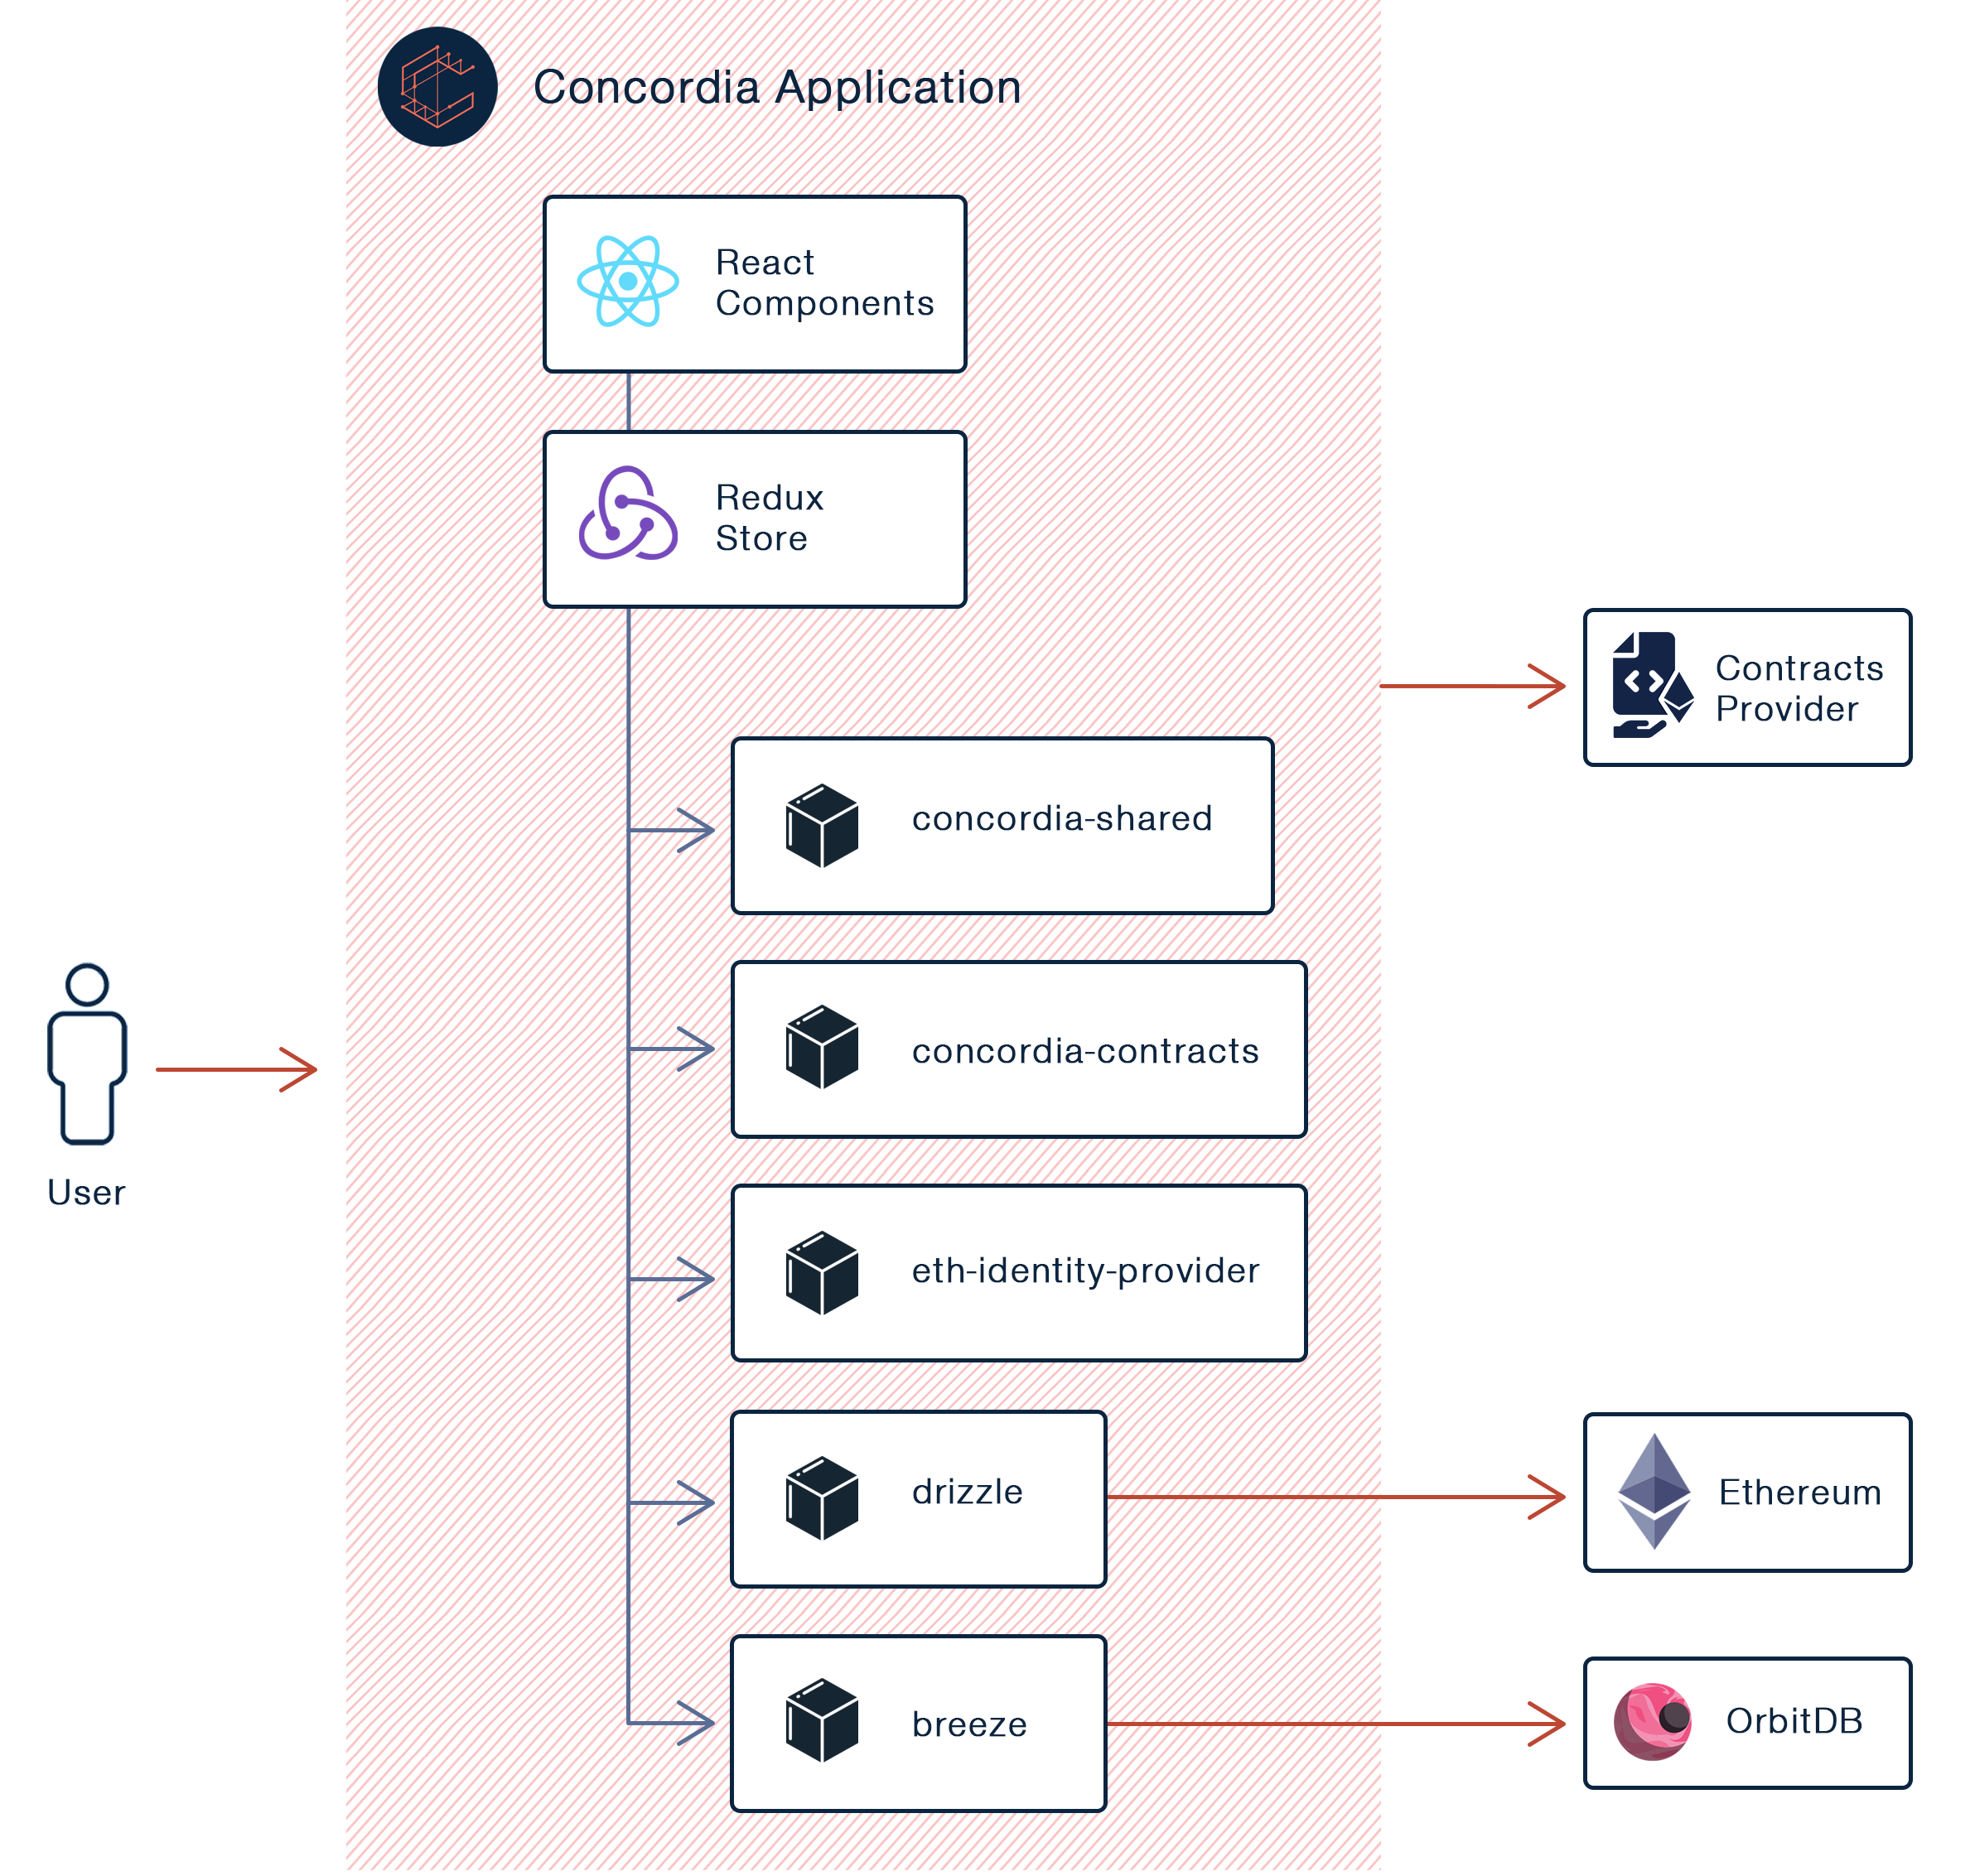
\includegraphics[width=.7\textwidth]{assets/figures/chapter-4/4.3.architecture-4.3.2.concordia-application-architecture.png}
    \caption{Αρχιτεκτονική υπηρεσίας Concordia Application}
    \label{figure:4-3-concordia-application-architecture}
\end{figure}

Για τη λειτουργία της υπηρεσία Concordia Application είναι απαραίτητα τα αντικείμενα (artifacts) που προκύπτουν από τη μεταγλώττιση των contracts και τη μεταφόρτωση/δημοσίευσή τους στο blockchain. Για την εισαγωγή των artifacts στην υπηρεσία έχουν αναπτυχθεί δύο μέθοδοι.

Η πρώτη μέθοδος είναι η μεταγλώττιση και μεταφόρτωση των contracts πριν την παραγωγή του πακέτου λογισμικού της υπηρεσίας για τελική χρήση (production build). Με αυτόν τον τρόπο η υπηρεσία θα έχει πρόσβαση στα artifacts μέσω της βιβλιοθήκης που παράγεται από το άρθρωμα concordia-contracts. Αυτή η μέθοδος έχει το μειονέκτημα ότι το τελικό πακέτο λογισμικού (production build) "δένεται" με όποια συγκεκριμένη έκδοση των contracts είναι διαθέσιμη κατά τη δημιουργία του πακέτου. Αυτό σημαίνει ότι σε ενδεχόμενη ενημέρωση των contracts πρέπει αναγκαστικά να δημιουργηθεί και νέα έκδοση του πακέτου λογισμικού της υπηρεσίας Concordia Application.

Για την αποφυγή του παραπάνω προβλήματος αναπτύχθηκε η δεύτερη μέθοδος προσκόμισης των contract artifacts, η οποία είναι η λήψη τους (download) από μία άλλη τοποθεσία στο διαδίκτυο. Σε αυτή τη μέθοδο, η εφαρμογή κατά την εκκίνησή της πραγματοποιεί ένα HTTP αίτημα (HTTP request) σε διεύθυνση η οποία δίνεται ως μεταβλητή περιβάλλοντος (environment variable). Η απάντηση του αιτήματος αναμένεται να περιέχει τα artifacts ώστε η εφαρμογή να τα χρησιμοποιήσει.

\subsubsection{Διανομή}

Η υπηρεσία Concordia Application πακετάρεται μαζί με τον διακομιστή nginx και γίνεται διαθέσιμη για χρήση ως εικόνα docker (docker image) μέσω του αποθετηρίου εικόνων dockerhub. Κατά την εκτέλεση της εικόνας οι χρήστες μπορούν μέσω μεταβλητών περιβάλλοντος να ορίσουν παραμέτρους της εκτέλεσης όπως η διεύθυνση του εξυπηρετητή (host location) της εφαρμογής και οι τοποθεσίες των υπηρεσιών Rendezvous Server και Contracts Provider.